%%%%%%%%%%%%%%%%%%%%%%%%%%%%%%%%%%%%%%%%%%%%%%%%%%%
%% P3: Phenomenology of Particle Physics                         
%%
%% Author:  André Rubbia                   		 
%%
%% Figure 11.12 Angular dependence in the center-of-mass frame of the differential cross-section
%% of the lepton pair creation process $e^+_Le^-_R \rightarrow\ell^+\ell^{-}$
%% and $e^+_Re^-_L \rightarrow\ell^+\ell^{-}$
%%
%% This work is licensed under the Creative Commons Attribution 4.0 International License. 
%% To view a copy of this license, visit http://creativecommons.org/licenses/by/4.0/ or 
%% send a letter to Creative Commons, PO Box 1866, Mountain View, CA 94042, USA.
%%
%%%%%%%%%%%%%%%%%%%%%%%%%%%%%%%%%%%%%%%%%%%%%%%%%%%

\documentclass[a4paper,10pt]{article}

\usepackage[T1]{fontenc}
\usepackage[utf8]{inputenc}
\usepackage{lmodern}
\usepackage[labelfont=bf]{caption}
\usepackage{upgreek}

\usepackage{tikz}
\usepackage{pgfplots}
\pgfplotsset{compat=1.17}
\usepgfplotslibrary{ternary}
\usepgfplotslibrary{fillbetween}
\usepgfplotslibrary{external}

\usepackage{braket}

\def\d{\mathrm{d}}

\begin{document}

%%%%%%%%%%%%%%%%% FIGURE %%%%%%%%%%%%%%%%%%%%%%%%%%%%%%%%%%
\begin{figure}[htb]
\begin{center}
\pgfplotsset{every axis/.append style={
    font=\large,
    line width=1pt,
    tick style={line width=0.8pt}}}
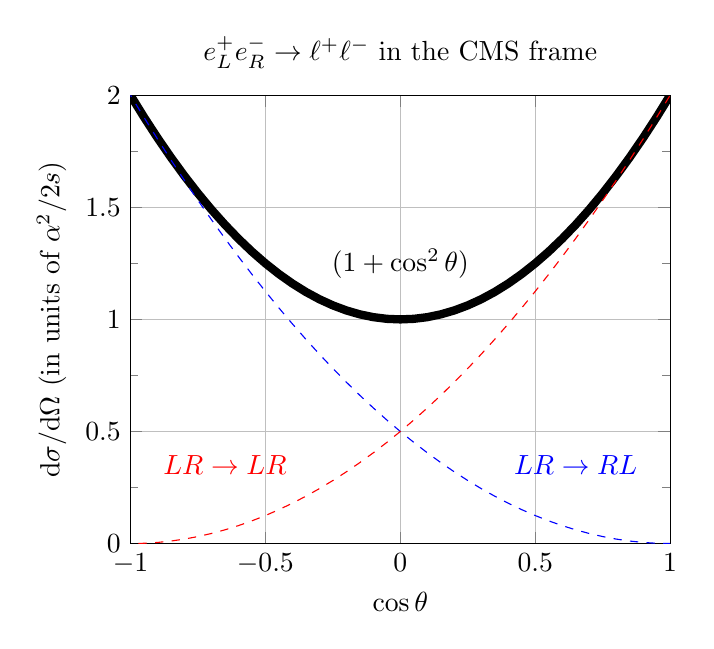
\begin{tikzpicture}[scale=1]
    \begin{axis}[
        title=$e_L^+e_R^- \rightarrow\ell^+\ell^{-}$ in the CMS frame,
        xlabel={$\cos\theta$},
        ylabel={$\d\sigma/\d\Omega$ (in units of $\alpha^2/2s$)},
        xmin=-1, xmax=1,
        ymin = 0, ymax=2,
        minor y tick num=1,
                grid = major
    ]
        \addplot [black,samples=201,  line width=3pt] {(1+x^2)};
        \addplot [blue,samples=201, dashed] {(1-x)^2/2};
        \addplot [red,samples=201, dashed] {(1+x)^2/2};
        \node[black] at (axis cs: 0,1.25) {$(1+\cos^2\theta)$};
        \node[red] at (axis cs: -0.65,0.35) {$LR\rightarrow LR$};
        \node[blue] at (axis cs: +0.65,0.35) {$LR\rightarrow RL$};
   \end{axis}
\end{tikzpicture}%
\\
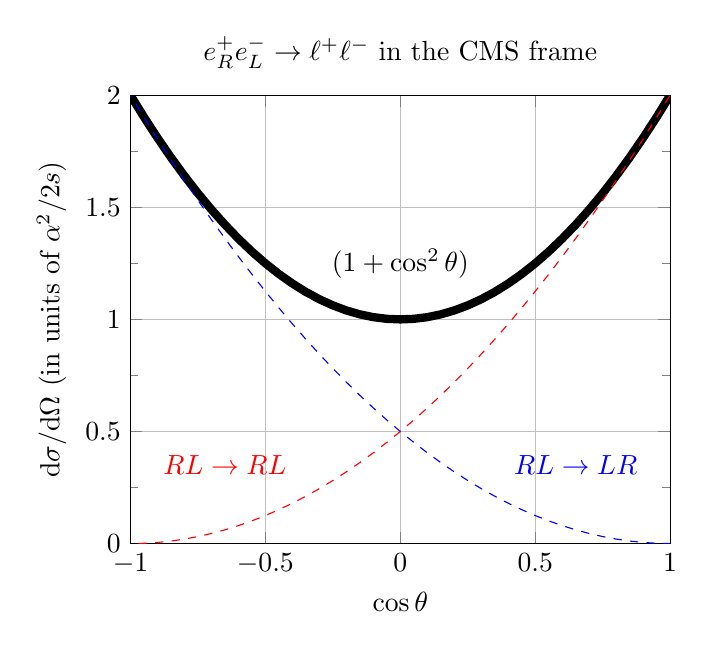
\begin{tikzpicture}[scale=1]
    \begin{axis}[
        title=$e_R^+e_L^- \rightarrow\ell^+\ell^{-}$ in the CMS frame,
        xlabel={$\cos\theta$},
        ylabel={$\d\sigma/\d\Omega$ (in units of $\alpha^2/2s$)},
        xmin=-1, xmax=1,
        ymin = 0, ymax=2,
        minor y tick num=1,
                grid = major
    ]
        \addplot [black,samples=201,  line width=3pt] {(1+x^2)};
        \addplot [blue,samples=201, dashed] {(1-x)^2/2};
        \addplot [red,samples=201, dashed] {(1+x)^2/2};
        \node[black] at (axis cs: 0,1.25) {$(1+\cos^2\theta)$};
        \node[red] at (axis cs: -0.65,0.35) {$RL\rightarrow RL$};
        \node[blue] at (axis cs: +0.65,0.35) {$RL\rightarrow LR$};
   \end{axis}
\end{tikzpicture}%
\caption{Angular dependence in the center-of-mass frame
of the differential cross-section
of the lepton pair creation process (top) $e^+_Le^-_R \rightarrow\ell^+\ell^{-}$
and (bottom) $e^+_Re^-_L \rightarrow\ell^+\ell^{-}$.}
\end{center}
\end{figure}
%%%%%%%%%%%%%%%%% END FIGURE %%%%%%%%%%%%%%%%%%%%%%%%%%%%%%
%

\end{document}
